\documentclass[french]{article}
\usepackage[T1]{fontenc}
\usepackage{babel}
\usepackage{hyperref}
\usepackage{graphicx}
\usepackage[justification=centering]{caption}
\usepackage{amsmath}
\usepackage{amssymb}

\hypersetup{
  colorlinks=true,
  linkcolor=black,
  urlcolor=blue
}

\graphicspath{ {./img/} }
\title{%
    \huge Apprendre à gagner au morpion grâce à l'apprentissage par renforcement  \\
    \bigskip
    \large E2 - Cas pratique 1 \\ 
    Développeur en Intelligence Artificielle,
    titre professionnel enregistré au RNCP - École IA Microsoft by Simplon}
\date{19 septembre 2023}
\author{par Vincent Papelard}

\begin{document}
    \maketitle
    \pagenumbering{arabic}
    \pagenumbering{gobble}
    \newpage
    \tableofcontents
    \newpage
    \pagenumbering{arabic}

    \section*{Introduction}
    Ce cas pratique se penche sur l'amélioration d'un modèle d'apprentissage par renforcement appliqué au jeu vidéo. Pour ce faire, nous allons partir d'un modèle que j'ai développé il y a quelques années. Son but ? Apprendre à jouer (et gagner !) à l'un des jeux les plus simples et les plus connus du monde : le morpion.
    
    Dans un premier temps nous ferons un état des lieux du modèle initial et de l'application qui lui est associée. Puis nous parlerons des outils utilisés dans le cadre de ce projet, avant d'étudier les solutions mises en oeuvre afin d'améliorer les performances de notre modèle.
    
    Le code associé à ce dossier est disponible sur GitHub : 
    \url{https://github.com/vinpap/tic_tac_toe}.
    \addcontentsline{toc}{section}{Introduction}

    \section{Situation de départ}
    \subsection{L'application}
    Tout d'abord, rappelons les règles du morpion. Deux joueurs s'affrontent sur une grille de 3x3 cases où ils choisissent une case à occuper à tour de rôle (l'un d'entre eux trace généralement des croix, et l'autre des cercles). L'objectif est de réussir à aligner trois de ses symboles à l'horizontale, à la verticale ou en diagonale, tout en empêchant son adversaire d'en faire autant. La partie s'arrête lorsque l'un des joueurs y parvient, ou si toute la grille est remplie (auquel cas la partie s'achève par un match nul). 

    L'application de départ est bâtie autour de plusieurs composants :
    \begin{itemize}
        \item Une classe qui implémente la logique des règles du jeu et gère le déroulement des parties
        \item Une classe qui affiche une interface graphique réalisée à l'aide du package Python PyGame. Celle-ci permet de visualiser en temps réel le déroulement des parties lorsque deux IA jouent ensemble, ou de jouer soi-même contre une IA
        \item Un ensemble de classes qui héritent d'une classe d'interface commune nommée PlayerInterface qui leur permet d'interagir avec le système de jeu. Dans la logique du programme, ces classes représentent des joueurs (humains ou IA) que l'on peut faire jouer en les enregistrant auprès du système de jeu à l'aide d'un simple appel de méthode. Cette structure nous permet d'ajouter facilement de nouveaux modèles d'IA à notre application.
    \end{itemize}

    \begin{figure}[h]
        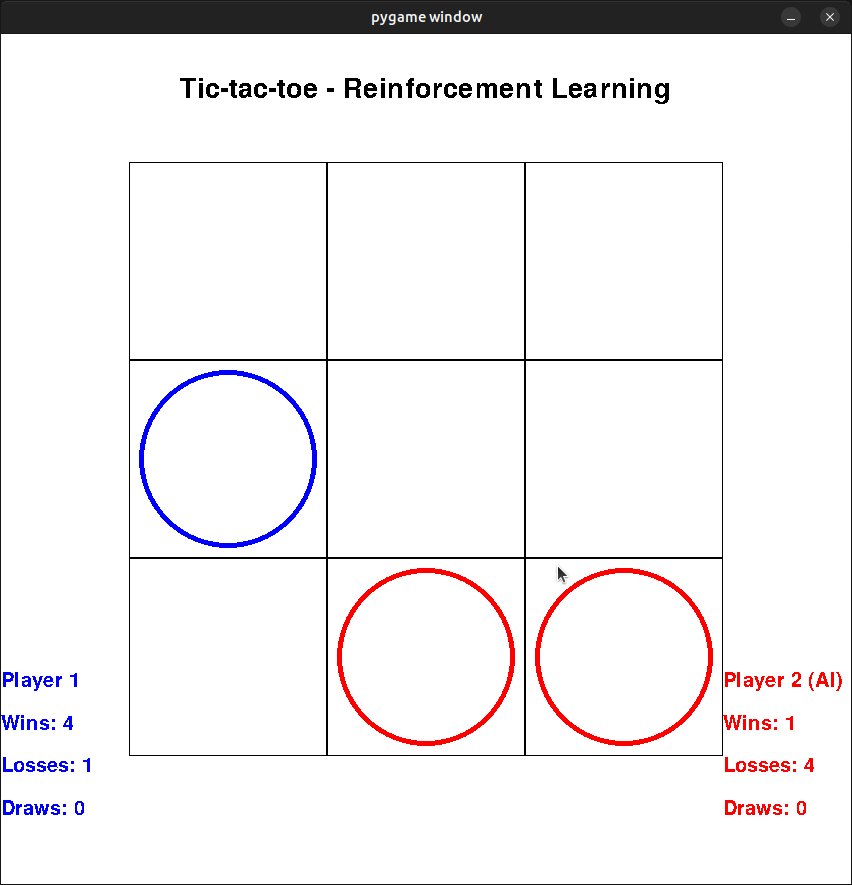
\includegraphics[width=7cm]{game_screenshot}
        \centering
        \caption{Une capture d'écran de l'interface du jeu, ici lors d'une partie entre un joueur humain et une IA}
        \centering
    \end{figure}

    \subsection{Le modèle}
    Le modèle initial pour ce projet est une implémentation du Q-learning, un modèle de renforcement dit "model-free". Commençons par parler du fonctionnement de ce modèle, et du renforcement de manière plus générale.

    \subsubsection{L'apprentissage par renforcement}
    L'apprentissage par renforcement (parfois abrégé RL pour "Reinforcement Learning" dans la suite de ce dossier) est l'un des grands paradigmes de l'apprentissage automatique. Avec cette méthode, le modèle est un agent qui cherche à optimiser une récompense quantitative au cours du temps à partir d'expériences dans un environnement donné. L'objectif d'un modèle de RL est d'ajuster son comportement, appelé politique ou stratégie. Pour mieux comprendre ces notions, voici à quoi correspondent ces différents concepts dans le cas qui nous intéresse :
    \begin{itemize}
        \item L'agent est notre modèle
        \item L'environnement est la configuration du plateau de jeu à un moment donné
        \item Une expérience est un coup joué 
        \item La récompense est le résultat à la fin d'une partie (victoire, défaite ou nul). Dans notre cas, on quantifie ce résultat en établissant qu'une victoire donne 1 point, un nul 0 et une défaite -1.
        \item La politique de notre modèle est la méthode qu'il utilise pour choisir un coup à jouer en fonction de l'état du plateau. La nature de cette politique varie selon les modèles, comme nous allons le voir.
    \end{itemize}

    Enfin, on notera qu'il existe deux types de modèles de RL : certains sont model-free, c'est-à-dire que notre IA n'a aucune connaissance préalable de l'environnement ou des mécanismes qui s'y produisent. D'autres sont model-based, ce qui veut dire qu'ils comportent un certain niveau de connaissance de l'environnement. Tous les modèles qui seront présentés ici sont model-free. Dit autrement, cela veut dire que nos modèles n'ont aucune connaissance des règles du morpion.
    
    Remarque: les principes de base du renforcement peuvent être facilement compris dans la mesure où ils sont inspirés des phénomènes d'apprentissage chez l'Homme et l'animal (se référer notamment à la célèbre expérience du \href{https://journals.openedition.org/bibnum/604}{chien de Pavlov}). On fait parfois une analogie entre le RL et certains aspects de l'éducation des enfants. Donner une récompense à un enfant, c'est encourager son comportement. Lui donner une punition (ou "récompense négative") c'est le dissuader de le reproduire.

    \subsubsection{Le Q-learning}
    Le Q-learning est l'un des algorithmes de RL les plus connus. Il tire son nom du fait qu'il est basé sur une fonction $Q:s * a \rightarrow \mathbb{R}$ qui calcule la valeur d'une paire état/action $(s, a)$, souvent appelée Q-value. Ici $s$ est l'état de l'environnement à un instant donné, et $a$ est une action possible dans cet état. Dit autrement, la Q-value définit la "qualité" d'une action à partir d'un état donné. Dans le cas du morpion :
    \begin{itemize}
        \item l'état Q est un vecteur à 9 dimensions qui est une visualisation aplatie du plateau à un moment donné. On représente les cases où l'IA a déjà joué par une valeur de 1, celles où son adversaire a joué par une valeur de -1, et les cases où personne n'a joué par une valeur de 0. À titre d'exemple, le plateau montré dans la figure 1 est représenté pour l'IA par le vecteur $\begin{bmatrix}0&0&0&-1&0&0&0&1&1\end{bmatrix}$.
        \item on représentera également une action comme un vecteur à 9 dimensions. Cette fois-ci, ce vecteur sera une représentation du plateau après avoir joué.
    \end{itemize}

    La Q-value de chaque action est stockée dans une table (appelée Q-table). Cette table constitue la politique du modèle de Q-learning, qui, pour faire un choix à un moment donné, choisira dans la table l'action qui présente la valeur la plus élevée pour l'état actuel.

    Une question centrale demeure : comment le modèle peut-il apprendre ces valeurs ? La réponse est apportée par l'équation de Bellman :
    \begin{align*} 
        V(s)=max_a(R(s,a)+ \gamma*V(s’))
    \end{align*}
    
    Cette fonction est à la base de plusieurs algorithmes de RL. Elle donne la valeur optimale d'un état, sans se pencher sur une action spécifique. Regardons-la plus en détail :
    \begin{itemize}
        \item $V(s)$ est un ŕéel qui donne la valeur d'un état $s$
        \item $s$ représente l'état
        \item $R(s, a)$ est la récompense immédiatement obtenue aprés avoir réalisé l'action $a$ dans l'état $s$
        \item $\gamma$ est le discount factor. C'est un paramètre de notre modèle compris entre 0 et 1 qui module l'impact de la valeur des états futurs potentiels sur les choix pris à un instant donné. Dit autrement, le modèle aura tendance à chercher des récompenses sur le long terme si l'on donne une valeur élevée à $\gamma$, et vice-versa
        \item $s'$ est l'état que le modèle atteindrait après avoir réalisé l'action s.
    \end{itemize}
    On pourrait verbaliser cette équation ainsi :

    {\centering \textbf{L'action optimale pour un état donné est celle qui maximise la somme de la récompense immédiate associée et de la valeur de l'état suivant pondérée par un facteur $\gamma$}}
    

    Remarque : il est tout à fait possible que certaines actions n'engendrent aucune récompense immédiate. Nous sommes dans ce cas : lors d'une partie de morpion, seul le dernier coup donne lieu à une récompense. C'est pour cette raison que la notion de "récompense immédiate" est absente des formules qui arrivent ci-dessous.
    
    On peut dériver l'algorithme du Q-learning de la notion de Q-value et de l'équation de Bellman. Celui-ci reste relativement simple :
    \begin{enumerate}
        \item Au début de l'entraînement, créer une Q-table qui contient toutes les actions possibles pour chaque état, et la remplir de valeurs arbitraires (0,5 dans mon cas)
        \item Puis on commence à jouer des parties contre un autre joueur (généralement une autre IA, pour pouvoir entraîner le modèle vite). À chaque tour, le modèle choisit soit de jouer le coup qui présente la Q-value la plus élevée, soit de jouer un coup au hasard. Ce choix représente le dilemne exploration vs exploitation et est conditionné par le paramètre $\epsilon$, deux éléments que nous aborderons plus après. 
        \item Au fil de la partie, le modèle garde en mémoire tous les coups qu'il a joués
        \item À la fin de la partie, il reçoit une récompense $r$ dont la valeur vaut -1, 1 ou 0. Il peut alors mettre à jour les Q-values stockées dans la table. Pour cela, il remonte l'historique des coups en partant de la fin et, assigne à chacun de ces coups une nouvelle Q-value comme suit :
        \begin{align*} 
            Q(s,a) := (1-\alpha)*Q(s,a) + \alpha(r + \gamma * max_a'(s',a'))
        \end{align*}
        où $max_a'(s',a')$ est la Q-value du coup disponible ayant la Q-value la plus élevée pour l'état suivant.
        
    \end{enumerate}

    Plus haut nous avons évoqué le dilemne exploration vs exploitation. Cette notion renvoit à un choix que tout modèle de renforcement doit faire lors de ses inférences : faut-il jouer le meilleur coup connu (i.e. exploiter ce que l'on sait déjà faire) ou tenter un nouveau coup aléatoire (et donc explorer d'autres possibilités) ? Ce choix est réalisé dans les modèles présentés dans ce dossier à l'aide de l'algorithme du epsilon-greedy. Celui-ci est très simple :
    \begin{itemize}
        \item À chaque inférence, le modèle choisit aléatoirement un réel entre 0 et 1
        \item Si ce nombre est supérieur à un paramètre $\epsilon$ fixé, alors on joue le meilleur coup connu
        \item Dans le cas contraire, on joue un coup aléatoire.
    \end{itemize}

    Le paramètre $\epsilon$ a donc un impact important : un epsilon trop bas peut rapidement conduire le modèle à stagner.

    En résumé :
    \begin{itemize}
        \item Le Q-learning est un modèle de renforcement basé sur une table qui contient les valeurs associées à chaque action possible pour chaque état
        \item L'algorithme d'entraînement est basé sur l'équation de Bellman
        \item Dans notre cas, le modèle s'entraîne en jouant des parties contre lui-même
        \item Lors de l'inférence, le paramètre $\epsilon$ est utilisé pour déterminer si le modèle va réaliser la meilleure action qu'il connaît ou effectuer une action aléatoire
        \item Les hyperparamètres du modèle sont le learning rate $\alpha$, le discount rate $\gamma$ et le facteur exploitation/exploration $\epsilon$.
    \end{itemize}


    \subsubsection{Performances de départ}

    Dans le cadre de notre projet, les performances du modèle sont mesurées lors d'une phase de test où on fait jouer notre modèle 100 parties contre un bot qui choisit tous ses coups aléatoirement. Le score $s$ est obtenu comme suit : 
    \begin{align*} 
        s = victoires - defaites
    \end{align*} 
    (les matchs nuls ne rapportent aucun point). Le modèle n'utilise pas le résultat de ces parties pour s'entraîner et choisira toujours de jouer les meilleurs coups connus (il ne cherchera donc pas à tenter de nouveaux coups). Cette phase de test est répétée régulièrement durant l'entraînement, en alternant 200 parties d'entraînement avec 100 parties de test.
    
    Voici les performances de notre modèle mesurées à différents points lors de l'entraînement, après avoir optimisé les hyperparamètres :

    \begin{figure}[h]
        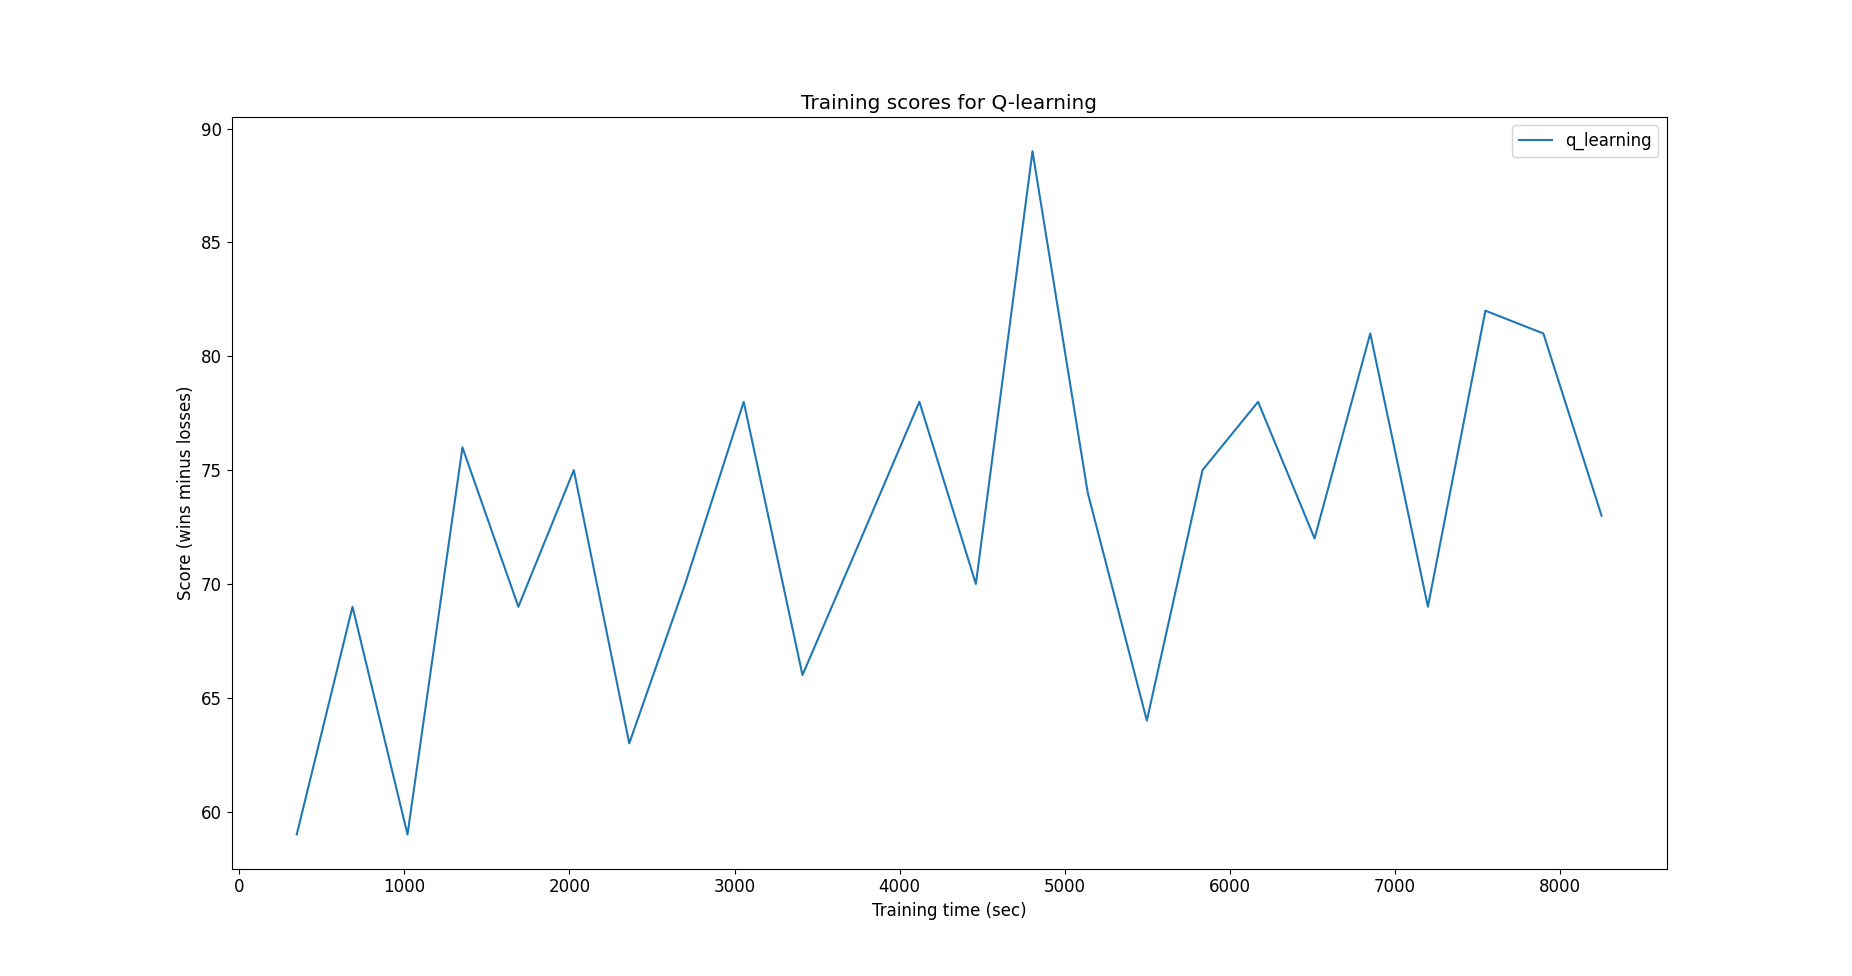
\includegraphics[width=12cm]{q_learning_metrics}
        \centering
        \caption{Évolution du score du modèle de Q-learning au fil de l'entraînement}
        \centering
    \end{figure}


    \section{Outils et méthodologie}
    \subsubsection{Gestion de projet}

    Afin de produire du code robuste et de vérifier la qualité du code produit, ce projet a été mené selon la méthode du Test-Driven Development. Dans le contexte de ce projet, cela consiste à coder les tests unitaires qui vérifient les performances et le bon fonctionnement des modèles produits avant de coder les modèles eux-mêmes.
    
    Voici un diagramme de Gantt qui présente l'estimation des charges réalisée en amont du projet :

    \begin{figure}[h]
        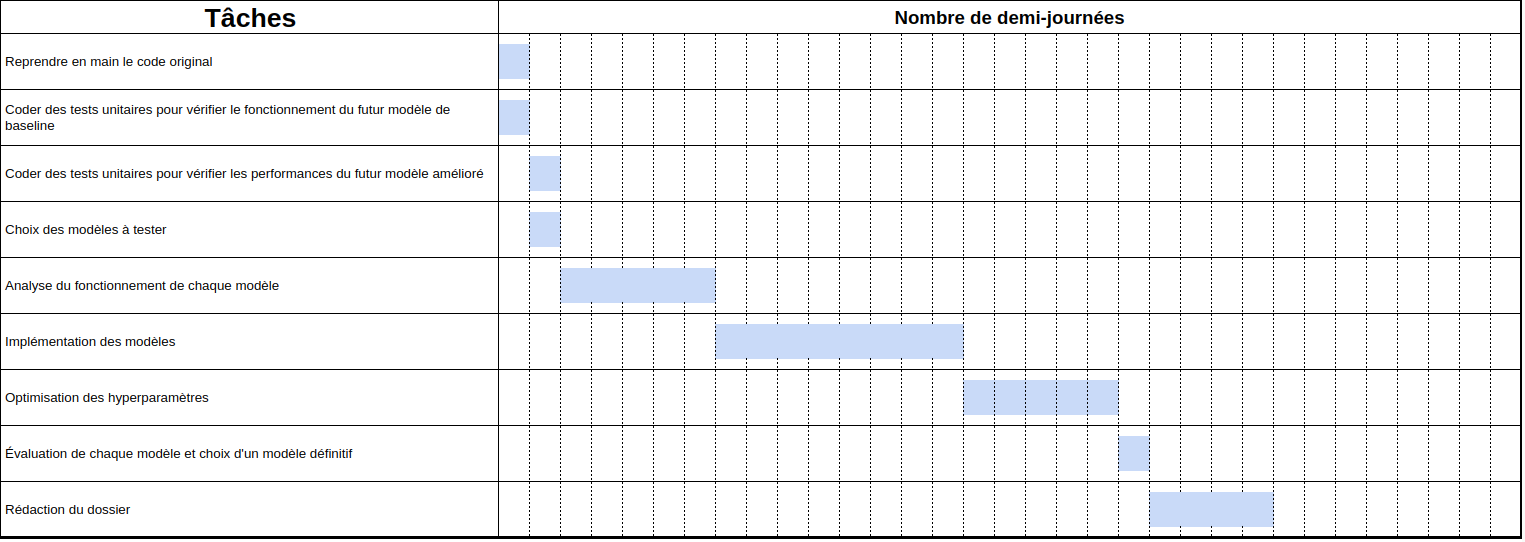
\includegraphics[width=13cm]{gantt}
        \centering
        \caption{Estimation de charge des différentes tâches du projet}
        \centering
    \end{figure}

    \subsubsection{Outils}

    Les outils utilisés pour ce projet sont les suivants :
    \begin{itemize}
        \item numpy
        \item keras
        \item pyGame pour l'interface
        \item pytest pour les tests unitaires
        \item GitHub pour le versionnement de code et la gestion des tâches
        \item \LaTeX pour la rédaction de ce rapport.
    \end{itemize}
    \subsubsection{Métriques}

    La métrique utilisée pour évaluer les différents modèles est le score présenté plus haut. Les temps d'entraînement de chaque modèle sont mesurés en secondes. 

    \section{Première tentative d'amélioration du modèle : le deep Q-learning}

    Dans la mesure où les hyperparamètres de notre modèle initial sont déjà optimisés, il paraît pertinent, pour améliorer les performances de notre IA, de changer de modèle. Dans cette optique, la première tentative d'amélioration choisie sera de remplacer notre modéle de Q-learning par un autre, le deep Q-learning.
    \subsubsection{Principe}

    Le deep Q-learning, comme son nom l'indique, partage beaucoup de caractéristiques avec le Q-learning. Il existe cependant une différence de taille entre les deux : alors que le q-learning tient une Q-table qui associe explicitement des valeurs à des paires (état, action), le deep Q-learning utilise un DNN pour prédire les Q-values. C'est ce type de modèle qui a été utilisé avec succès par Deepmind pour créer des IA capables de jouer à des jeux Atari.


    \subsubsection{Implémentation}
    Voici la structure du réseau utilisé dans notre implémentation de deep q-learning :
    \begin{figure}[h]
        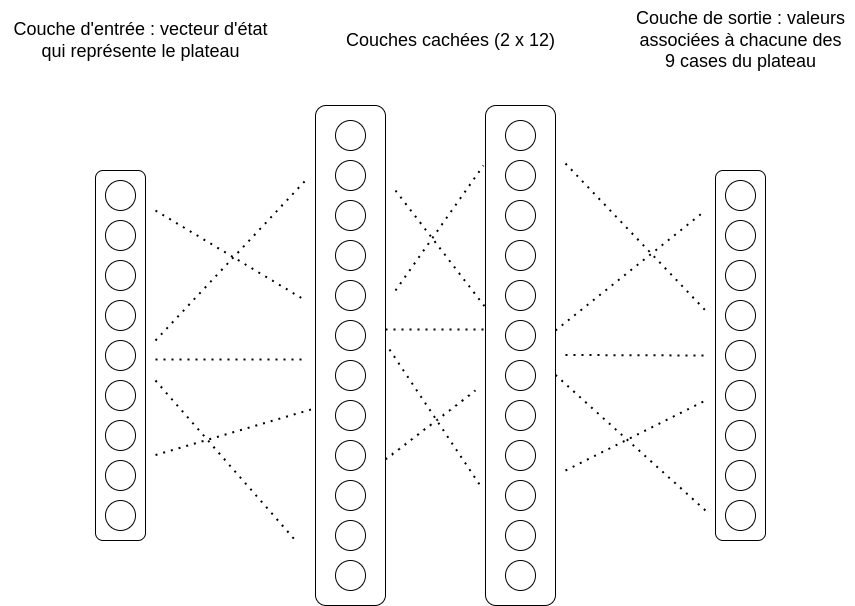
\includegraphics[width=13cm]{structure_dnn}
        \centering
        \caption{Structure du réseau utilisé par le deep q-learning}
        \centering
    \end{figure}

    Ici, notre réseau prédit la Q-value associée à chaque coup possible pour l'état donné en entrée du réseau.

    Pour entraîner ce modèle, on garde un historique des coups joués appelé replay buffer. À intervalles réguliers, on réentraîne notre réseau comme suit :
    \begin{enumerate}
        \item on sélectionne aléatoirement des coups dans le buffer
        \item pour chacun de ces coups, on réentraîne notre réseau. Pour obtenir le vecteur de sortie attendu en sortie de notre réseau, on réalise une inférence avec le réseau puis on remplace la dimension du vecteur correspondant au mouvement joué par la valeur calculée grâce à l'équation de Bellman.
    \end{enumerate}

    \subsubsection{Résultats}

    Une comparaison des performances du q-learning et du deep q-learning après optimisation du learning rate est présentée est la figure 5.
    
    \begin{figure}[h]
        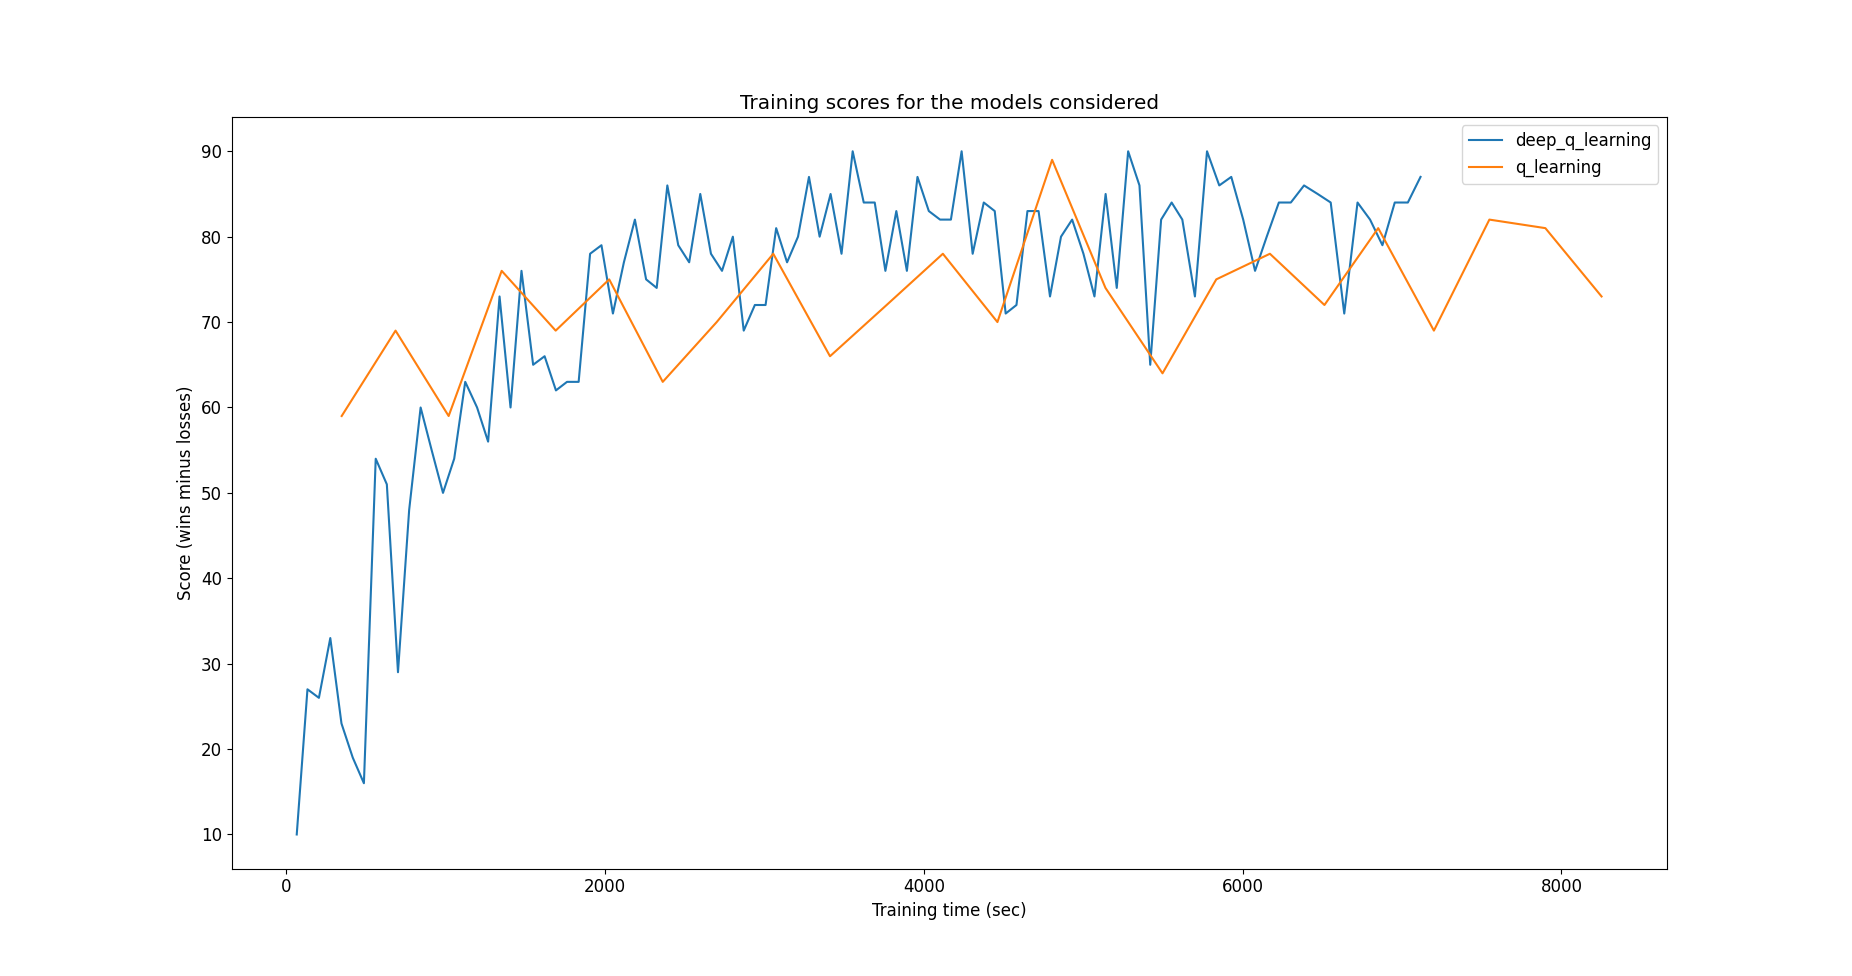
\includegraphics[width=12cm]{deep_q_learning_metrics}
        \centering
        \caption{Comparaison des scores du Q-learning et du deep Q-learning}
        \centering
    \end{figure}

    On constate une légère amélioration des performances. Cependant il est possible de mieux faire !

    \section{Deuxième tentative d'amélioration du modèle : modification du modèle de Q-learning pour utiliser un learning rate variable}

    \subsection{Principe}

    En observant la courbe qui décrit les performances du modèle d'origine, on remarque que le score fluctue beaucoup d'une phase de test à une autre, et modifier le learning rate n'a pas permis d'améliorer le score. Cependant, cette réflexion a engendré une nouvelle idée : Faire varier le learning rate durant l'entraînement permettrait-il d'améliorer les performances ? Intuitivement, on pourrait en effet penser que commencer l'entraînement avec un learning rate de 1 et le réduire progressivement pourrait permettre au modèle d'apprendre vite au début, puis d'ajuster ses q-values par petites touches par la suite.

    Cette méthode est surprenamment simple à mettre en place. Reprenons la formule utilisée pour mettre à jour la Q-table dans le modèle d'origine :
    \begin{align*}
        Q(s,a) := (1-\alpha)*Q(s,a) + \alpha(r + \gamma * max_a'(s',a'))
    \end{align*}

    Notons que cette assignation ne correspond à rien d'autre que la moyenne de la Q-value existante et de la nouvelle valeur calculée pour le coup considéré, de coefficients $\alpha$ et $-\alpha$. Introduisons maintenant un entier positif $n$ qui désigne le nombre de fois qu'un couple (état, action) donné a été rencontré. Enregistrons et mettons à jour cette valeur pour chaque coup au fil de l'entraînement, puis remplaçons la formule précédente par celle-ci :
    \begin{align*}
        Q(s,a) := \frac{n*Q(s,a) \:+ \:r \:+ \:\gamma * max_a'(s',a')}{n\:+\:1}
    \end{align*}

    ou, vu autrement, si on note $Q_n$ la Q-value d'une action jouée $n$ fois, la Q-value d'une action à un moment donné est caractérisé par $Q_n(s,a) = \overline{Q(s,a)}$.

    \subsection{Implémentation}

    L'implémentation de cette modification est relativement rapide : il a suffi de modifier quelques lignes de code dans la fonction qui actualise la Q-table et de modifier le format de cette dernière pour qu'elle stocke, pour chaque paire état-action, le nombre de fois où cette configuration a déjà été rencontrée durant l'entraînement.
    \subsection{Résultats}

    Voici les résultats obtenus avec cette méthode comparés à ceux des modèles précédents :


    \begin{figure}[h]
        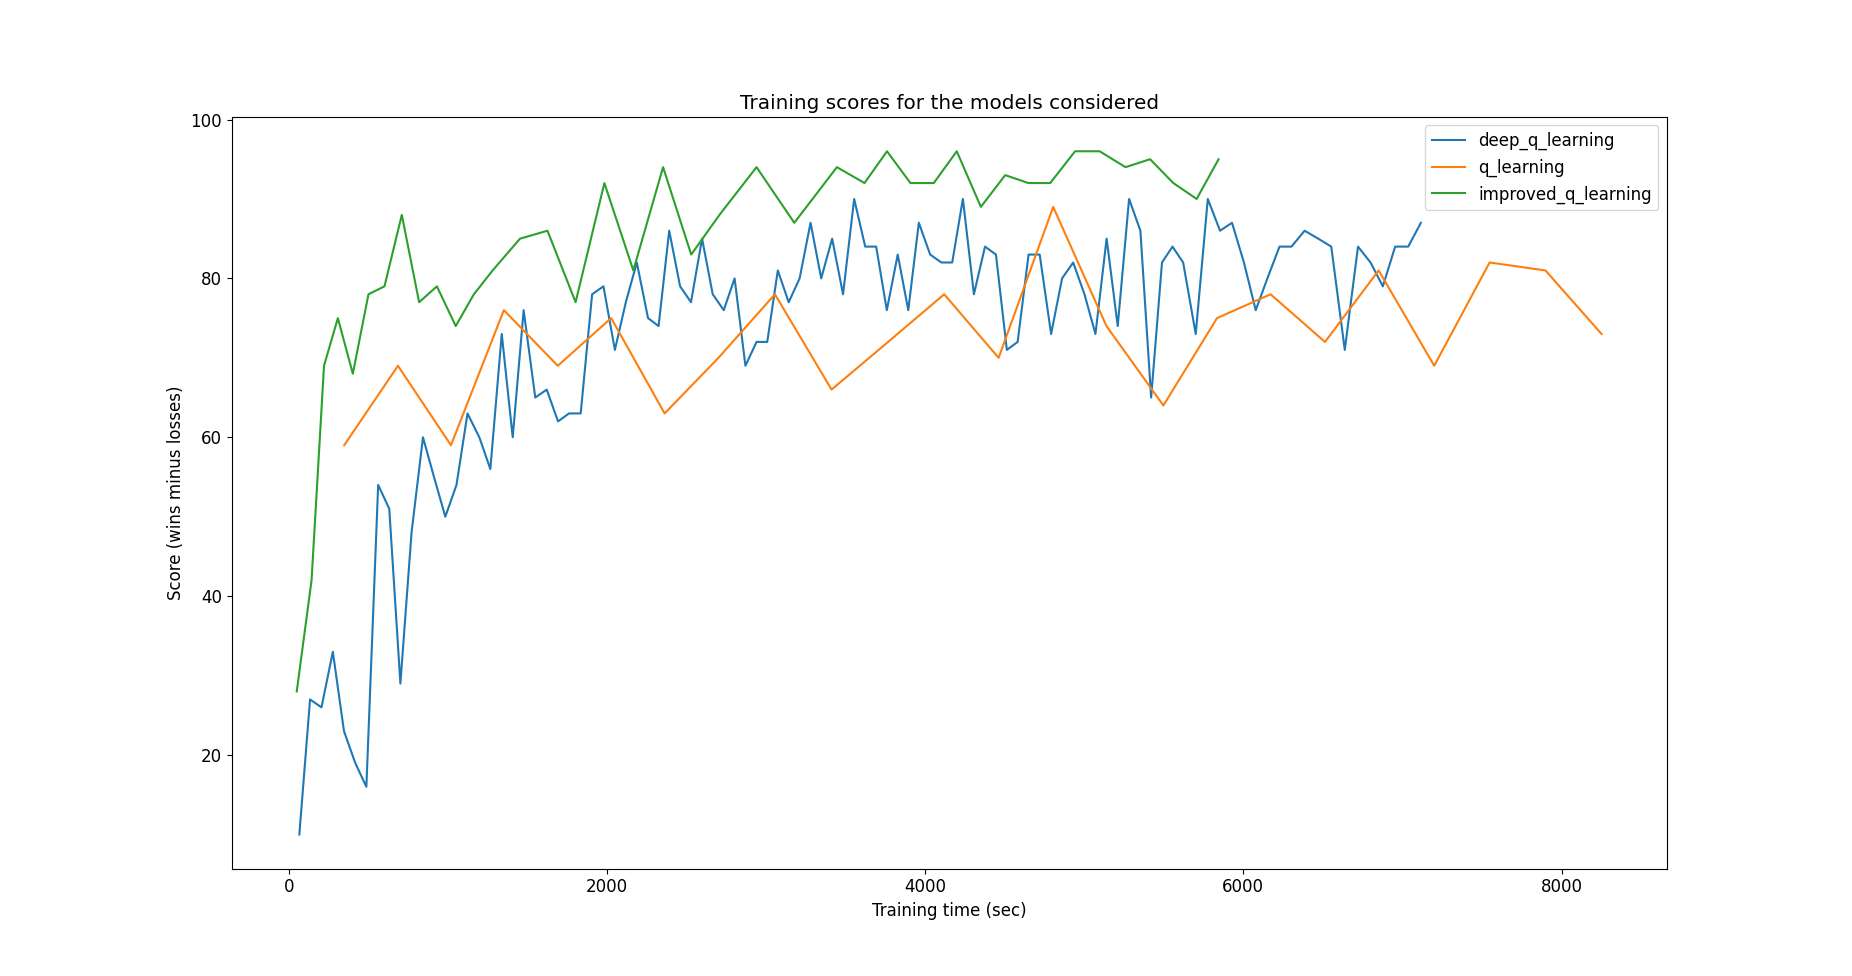
\includegraphics[width=12cm]{improved_q_learning_metrics}
        \centering
        \caption{Comparaison du score du modèle de Q-learning modifié avec les modèles précédents}
        \centering
    \end{figure}

    On remarque cette fois-ci une amélioration nette des résultats, avec un score supérieur à 90 en fin d'entraînement. Utiliser un learning rate variable était donc une bonne idée.
    
    \section{Bilan et leçons à tirer}
    \subsection{Rétrospective sur la gestion de projet}

    Voici un diagramme qui compare les charges de travail estimées au début de ce dossier et le temps réellement passé sur chacune des tâches du projet :

    \begin{figure}[h]
        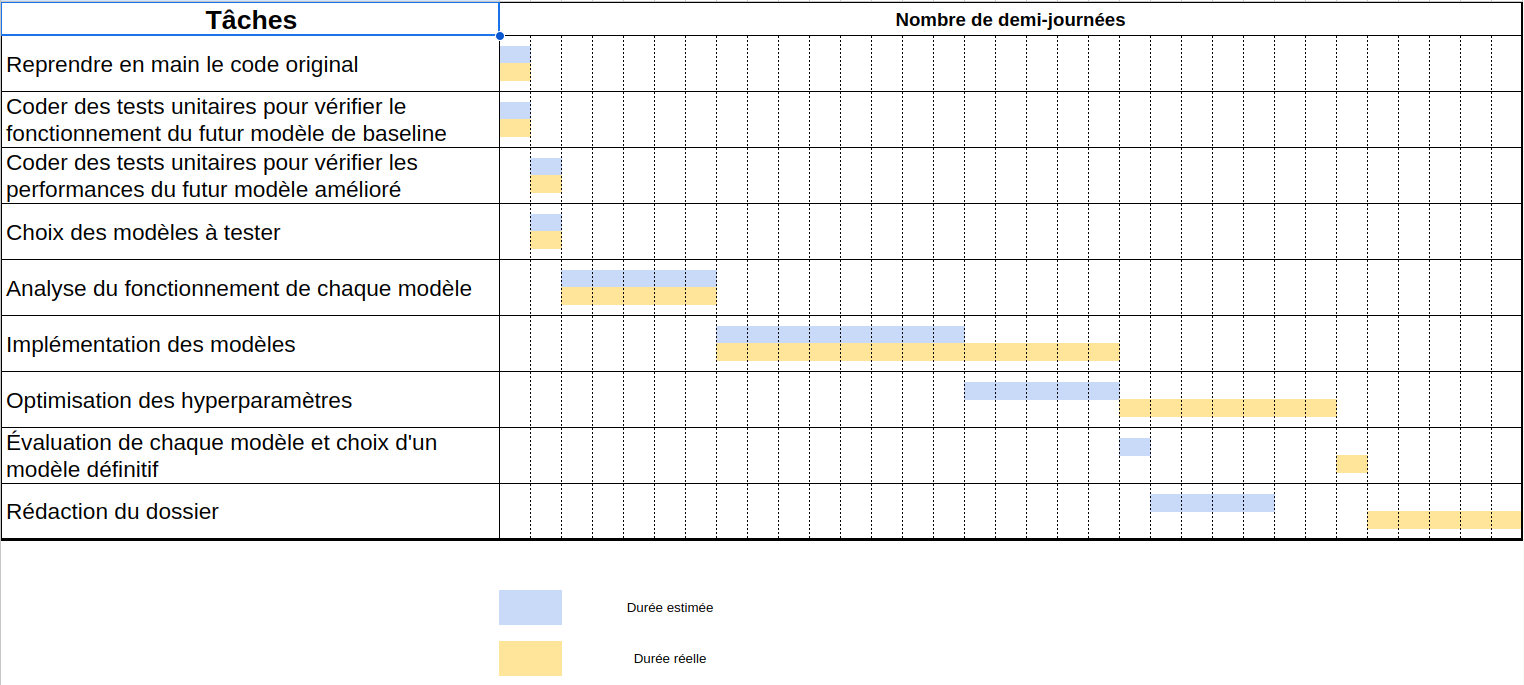
\includegraphics[width=13cm]{gantt_2}
        \centering
        \caption{Comparaison entre l'estimation des charges initiale et le temps réellement passé sur les différentes tâches du projet}
        \centering
    \end{figure}

    Si le temps passé sur les premières tâches du projet a bien été estimé, celui nécessaire pour implémenter et optimiser les différents modèles a été largement sous-estimé. Cela s'explique par plusieurs facteurs qui seront détaillés ci-dessous.

    \subsection{Les grandes difficultés rencontrées}

    Comme nous venons de le dire, la première difficulté rencontrée concerne le temps de travail nécessaire pour travailler sur ce projet, largement supérieur à ce qui était initialement estimé. Ceci s'explique par deux facteurs :
    \begin{itemize}
        \item Les modèles de renforcement sont plus difficiles à mettre en place que les modèles d'apprentissage supervisé ou non supervisé. Alors qu'il est souvent possible de trouver des implémentations prêtes à l'emploi de ces derniers, l'implémentation d'un modèle de renforcement dépend en large partie du problème spécifique auquel ce dernier doit répondre. Par conséquent les modèles de renforcement présentés dans ce dossier ont dû être codés à partir de zéro, d'où un temps de travail plus long.
        \item Les modèles de renforcement sont connus pour être longs à entraîner. C'est pour cette raison que l'optimisation des hyperparamètres a été si longue : chaque entraînement prenant plus de deux heures, plusieurs jours ont été nécessaires pour tout optimiser.
    \end{itemize}

    Une autre difficulté concernant ce projet est liée au fait même d'utiliser des modèles de machine learning pour résoudre un problème tel que celui-ci. Même si le modèle amélioré affiche des performances respectables, il n'en reste pas moins qu'il a fallu entraîner un modèle pendant plusieurs heures. Or, le jeu du morpion est un jeu où il existe un nombre de configurations de plateau possibles relativement limité, et certains algorithmes ne faisant pas appel au machine learning tels que le minimax peuvent déjà résoudre ce problème. On pourra donc discuter de la pertinence du machine learning pour résoudre ce problème en premier lieu.

    \section{Conclusion}

    Au final, ce projet aura été l'occasion d'explorer un pan du machine learning peu abordé jusque-là dans le cadre de la formation. L'apprentissage par renforcement offre pourtant de nombreuses possibilités, dans le développement d'IA liées au jeu vidéo mais aussi en robotique, en vision par ordinateur ou dans le cadre du finetuning d'un LLM tel que GPT-3. 

    L'application du RL à un problème simple tel que le morpion m'a permis de m'initier à ce paradigme et j'espère pouvoir bientôt exploiter toutes les possibilités du renforcement dans d'autres contextes.

    \section*{Bibliographie}
    \addcontentsline{toc}{section}{Bibliographie}

\end{document}